\fancyhead[LE,RO]{Sucrose inversion -- ,,ELS''}
\fancyhead[LO,RE]{\thesection}
\fancyfoot[LE,RO]{\thepage}
\fancyfoot[RE,LO]{\emph{Physical chemistry lab. practice for pharmacy students}}

%\setcounter{section}{7}
\section{Investigation of sucrose inversion with polarimetry}
\subsection{Introduction}
The purpose of the studies in reaction kinetics is to reveal the underlying mechanisms, for which the knowledge of the order or partial order regarding the reactants is really helpful.
The general rate equation for homogeneous reactions is:

\begin{equation}
\label{eq:general}
	r
	=
	k[A]^{\beta_a}[B]^{\beta_b}...[N]^{\beta_n}
\end{equation}

where $\beta_a$, $\beta_b$ and $\beta_n$ are the partial order of the respective reactants, and $\beta = \beta_a + \beta_b + ... + \beta_n$ is the overall order of the reaction.

If there is concentration -- time data available and we know the order of the reaction, the rate constant can be calculated.

\paragraph{Using the rate equations.}
It is possible to use the indefinite integral form of first order reactions for graphical evaluations:

\begin{equation}
\label{eq:2}
	\ln 
	\frac{[A]}{[A]_0}
	=
	- k
	t
\end{equation}

Plotting $\ln [A]$ as a function of time we get a staright line, whose slope is $-k$, the rate constant (fig. \ref{fig:els_1}). Note that the slope of the $\ln ([A]/[A]_0) - t$ and $\ln [A] - t$ functions are the same, since $\ln ([A]/[A]_0) = \ln [A] - \ln [A]_0$ and $\ln [A]_0$ is constant.

\begin{figure}[b]
\centering
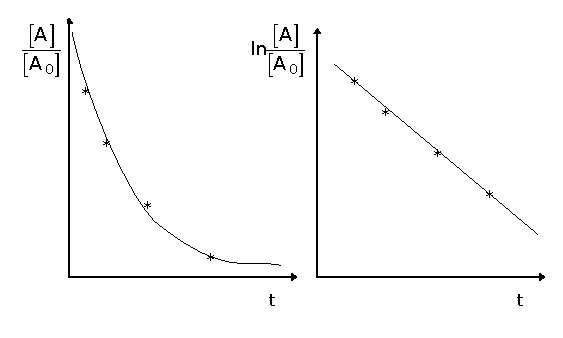
\includegraphics{els1.eps}
\caption{Determining the rate constant of a first order reaction.}
\label{fig:els_1}
\end{figure}

Usually concentration is not measured directly, but a quantitiy that is proportional to concentration is measured. We will denote this quantitiy as $z$ in general.
It is easy to see that the difference between $z_0$ at time $t = 0$ and $z_\infty$ at time $t = \infty$ is proportional to $[A]_0$ and the product concentration at the end of the reaction ($t = \infty$), if there is a linear relationship between $z$ and $[A]$.
Then, it is possible to express the concentration $[A]$ at any time $t$ if the measured signal $z_t$ at time $t$ and $z_{\infty}$ is known.
Substituting to eq. \ref{eq:2}, we get

\begin{equation}
\label{eq:3}
        \ln 
        \frac{z_{\infty}-z_t}{z_{\infty}-z_0}
        =
        - k
        t
\end{equation}


\paragraph{Guggenheim's method.}
To use eq. \ref{eq:3}, to determine the rate constant of a first order reaction, the knowledge of the physical parameter $z$ at both $t=0$ and $t=\infty$ is necessary.
When the reaction is too fast or too slow however, measuring $z_0$ or $z_\infty$ might prove to be problematic due to technical difficulties.
To circumvent these difficulties one could use \emph{Guggenheim's method}. To do this, measure $z_t$ at $t_1, t_2, t_3, ... , t_n$ and at $t_1+\Delta t, t_2+\Delta t, t_3+\Delta t, ... , t_n+\Delta t$, where $\Delta t$ is a constant time interval.
For instance if we measured $z$ at $t= 12, 18$ and $27$ seconds, and $\Delta t = 30 s$, we measure $z$ at 42, 48 and 57 seconds as well.

\begin{figure}[h]
\centering
\label{fig_els2}
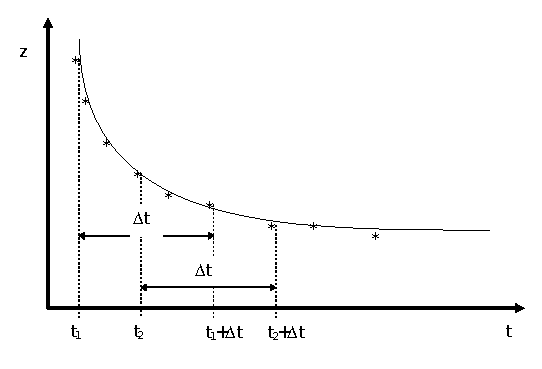
\includegraphics{els2.eps}
\caption{Determining the rate constant of a first order reaction using \emph{Guggenheim's method}.}
\end{figure}

First we substitute $t$ and $t + \Delta t$ into the exponential form of eq. \ref{eq:3}, then rearrange the resulting equation:

\begin{equation}
\label{eq:4}
	z_t - z_{\infty}
	=
	(z_0 - z_{\infty}) e^{-kt}
\end{equation}

\begin{equation}
\label{eq:5}
	z_{t + \Delta t} - z_{\infty} = (z_0 - z_{\infty}) e^{-k(t+\Delta t)}
\end{equation}

Then substract eq. \ref{eq:5} from \ref{eq:4} to get

\begin{equation}
\label{eq:6}
        \ln (z_t - z_{t+\Delta t})
	=
	-kt
	+ \ln (z_0 - z_{\infty}) (1- e^{-k \Delta t})
\end{equation}

The second term on the right side is constant, since $z_0$ and $z_\infty$ does not change during the reaction (we don't add or remove reactants or products), and $\Delta t - t$ was chosen to be constant.
Thus, if we plot the left side as a function of $t$, we get a linear equation, whose slope is $k$, the rate constant.
Notice that for this method to work, we don't need to know either $z_0$ nor $z_\infty$. 
It must be mentioned however that one should choose $\Delta t$ carefully, preferably it should be as big as possible.
The estimation will be more precise if we measure in a small range of conversion, and $\Delta t$ approaches the half life ($t_{1/2}$) of the reaction.

\paragraph{Method of initial rates.}
Usually it's not possible to follow the concentration changes of all components in a reaction, nevertheless, the reaction order and rate constant is possible to measure anyway. Let's take a logarithm of both sides of eq. \ref{eq:general}: 

\begin{equation}
\label{eq:log}
	\ln r
	=
	\ln k
	+ \beta _a \ln [A]
	+ \beta _b \ln [B]
	+ ...
	+ \beta _n \ln [N]
\end{equation}

If we keep the concentration of every component constant except for example $A$, and we measure the rate constant at several different $[A]_0$, the we get a linear equation when we plot $\ln r$ as a function of $\ln [A]_0$. The slope of this equation is $\beta _a$, the partial order with respect to $A$.
This is true only at low conversion range, ie. the initial part of the reaction. The measurements must be done at time instances when $t << 0.05 t_{1/2}$.

\subsection{Investigating the inversion reaction of sucrose}
Sucrose is a disaccharide, which undergoes hydrolysis in acidic medium. As a result, D-glucose and D-fructode are being produced:

\begin{equation}
\label{eq:inversion}
	C_{12}H_{22}O_{11} + H_2O = C_6H_{12}O_6 + C_6H_{12}O_6
\end{equation}

If the solution is dilute enough, this becomes a pseudo first order reaction, because the ,,concentration of water'' does not change significantly.
The reaction occures in neutral solutions as well, but very slowly. Dilute acids will catalyse the reaction, and the reaction rate will be proportional with the concentration of the acid.
Since the reaction can be regarded as first order reaction, with eq. \ref{eq:3} the rate constant can be calculated if we measure a physical parameter that is proportional with the concentration of any of the components in the reaction.
In this practice we will use rotation of light that is passing through the solution.
In our system there are several optically active components: the solution of sucrose rotates light to the right ($+$), the products rotate light to the left ($-$).
This phenomenon is a result of the chirality of chemical compounds.
The speed of light in the optically active media is different for light polarized to the right and left.
Thus, there is a shift in phase when light hits the detector. If we use \emph{polarized} light, there is only light with a certain rotational angle, and it's possible to measure the phase shift.

In a cuvette with a length $l$, rotation is defined by

\begin{equation}
\label{fig:rotation}
	\alpha
	=\frac{10 \pi l}{\lambda}
	(n_l -  n_d)
\end{equation}

where $\lambda$ is the wavelength of light in cm, $n_l$ is the refractive index of light polarized to the left, $n_d$ is that of light polarized to the right.
Specific rotation is the rotation angle which is observed in a solution with a concentration of 1 g/cm$^3$ when $l = 1$ dm.
Since rotation depends on waveength and temperature, usually it is referenced to the \emph{D line} of sodium for either 20 or 25 $\celsius$.


\subsection{Practice procedures}
Prepare 100 cm$^3$ 30 m/m\% sucrose solution and 50 cm$^3$ 5 M HCl. To have a complete reaction at the end of the practice, first assemble the following reaction: 10 cm$^3$ sucrose solution $+$ 10 cm$^3$ HCl. Put it in a 50 $\celsius$ thermostat. By the end of the practice, the reaction should have been undergone completely. Leave it there for now, and continue with the $t = 0$ solution. Do this by creating a solution of 10 cm$^3$ sucrose solution $+$ 10 cm$^3$ H$_2$O. In this solution the reactions proceeds quite slowly, and it will not change significantly during the practice. This is the initial state, since there is only sucrose in the solution, and no glucose or fructose. You can take your time and familiarize yourself with the polarimeter.

Turn on the \emph{Krüss P1000-LED} polarimeter. This instrument is using LEDs as light source, therefore there is no need for warmup. Ask the instructor or the technician if you don't know how to use it. Measure the rotation of light in the $t = 0$ solution. Start recording in such a table:

\begin{center}
\begin{tabular}{|c|c|c|c|c|}
\hline
$t$, minutes & $z$, degrees \\
\hline
... & ... \\
\end{tabular}
\end{center}
 
Prepare 2 of reaction mixtures from table \ref{table:reactions} (ask the instructor which 2).

\begin{table}
\caption{Reaction mixtures to study sucrose inversion as a function of time.}
\centering
\begin{tabular}{cccc}
%\hline
\# & sucrose solution, ml & HCl solution, ml & deionized water \\
\hline
1 & 10 & 10 & 0 \\
2 & 10 & 8 & 2 \\
3 & 10 & 5 & 5 \\
4 & 10 & 2 & 8 \\
\end{tabular}
\label{table:reactions}
\end{table}

Prepare the solutions in a large enough, clean beaker. Stir the mixture thoroughly and start the stopwatch when you pour tha last component into the beaker (it should be the sucrose or the HCl solution, but NOT water). This is when the reaction starts. Then quickly fill the cuvette of the polarimeter with the reaction mixture and put it into the polarimeter (don't forget the caps). Start reading rotational angles at a 60, or if you can handle it a 30 s interval. Write down in the table the time and the angle at that time. Collect altogether 25 points for each reactions.

\subsection{Evaluation}
Evaluate the collected data according to this table:

\begin{center}
\# of reaction: ... , $z_0 = ...$ degrees, $z_\infty = ... $ degrees
\begin{tabular}{|c|c|c|c|c|}
\hline
$t$, minutes & $z_t$, degrees & $z_t - z_\infty$ & $\ln(z_0-z_\infty)- \ln(z_t-z_\infty)$, degrees & $k$, 1/s \\
\hline
... & ... & ... & ... & ... \\
\end{tabular}
\end{center}

Plot the 4th column as a function of time $t$, and determine $k$ graphically as well.
Calculate $k$ with Guggenheim's method too. Choose at least 15 minutes for $\Delta t$. 
Plot $\ln (z_t - z_{t+\Delta t})$ as a function of $t$, and determine $k$ from the slope.

